\section{Hjerteudredning}
Hjertekarsygdomme er, som navnet antyder, sygdomme der optræder i hjerte og/eller blodkar. Af sygdomme i hjertet kan der som eksempel nævnes hjerteklapfejl, hjertesvigt og forkammerflimmer. Åreforkalkning er en karsygdom der kan give indsnævring i blodårene og dermed reduceret blodgennemstrømning. Dette kan lede til en blodprop, der kan i princippet opstå overalt i kroppen, f.eks. i hjertet, hjernen, benene eller lungerne. Symptomerne ved hjertekarsygdomme afhænger af det berørte organ, dog i nogle tilfælde kan patienten være symptomfri. Det kræver derfor en grundig lægeundersøgelse for at afklare diagnose og behandlingsbehov \cite{apoteket}. 

Ved den praktiserende læge er hjerteudredning bygget på objektiv undersøgelse og patientens sygdomshistorik. Nogle gange vælger lægen at lave en længerevarende monitorering, hvor patienten får et måleapparat med hjem. Hvis den praktiserende læge vurderer at en patient har begrundet mistanke om en eller anden form for hjertesygdom, vil han give henvisning til en hjertespecialist. Afhængigt af symptomerne anvendes der herefter en række forskellige laboratorieteknikker til diagnosticering. I akutte tilfælde bliver patienten dog indlagt med det samme \cite{hjerud}. Et overblik over diagnoseringsforløbet kan ses på \ref{fig:forloeb}, og underpunkterne bliver nærmere forklaret i kommende afsnit.

\begin{figure}[H] % Example of including images
\begin{center}
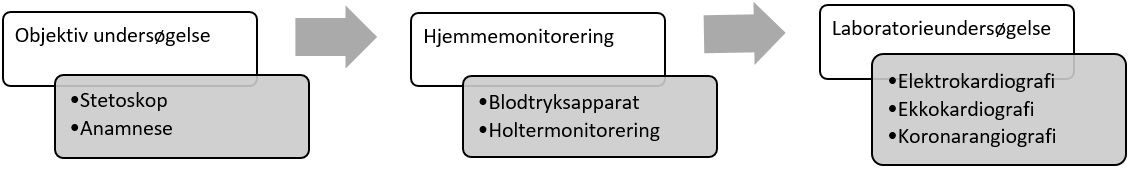
\includegraphics[width=1\textwidth]{figures/forloeb}
\end{center}
\caption{Overblik over diagnoseringsforløbet af hjertekarsygdomme}
\label{fig:forloeb}
\end{figure}

\subsection{Objektiv undersøgelse}
Ved tidlig mistanke om et kardiovaskulært problem, kan lægen anvende et stetoskop til at lytte på hjertet \cite{subob}. Hjertelydene identificeres efter rytme, første- og anden hjertelyd, systole og diastole samt mislyde. Disse giver lægen mulighed for at identificere hvilken del af hjertet der er eventuelle komplikationer med. Ved måling med et stetoskop skal lægen manuelt lytte på patientens hjerte og selv vurdere om eventuelle hjertefejl, hvilket kræver at lægen skal have nogen erfaring med dette [KILDE???!]. Herudover vil lægen spørge patienten ind til symptomerne, risikofaktorer og dens families evt. sygdomshistorie \cite{hjerud}. 
 
\subsection{Laboratorieundersøgelse}
I laboratoriet undersøger specialisten hjertets elektriske aktivitet (som blev beskrevet i afsnit \ref{Hjertets_elektriske_ledningssystem}) vha. en elektrokardiografi, hvilket giver udtryk for i hvilken grad hjertets evne til at slå er intakt \cite{ekg}. EKG-signalet giver et billede af hjertets evne til at lede elektrisk strøm til hjertemuskulaturen, men dog ikke i hvor effektivt hjertet er til at flytte blodet. Ved at måle EKG kan lægen dermed finde ud af om en eventuelt fejl på hjertet skyldes problemer med den elektriske ledning \cite{ekg}.
 
Hvis komplikationerne vedrørende hjertet ikke er elektriske relaterede, kan hjertets blodtilførelse undersøges gennem et ultralydsapparat – denne metode kaldes ekkokardiografi (EKKO). Undersøgelsen giver information om, hvordan hjertet er bygget op, og hvordan de enkelte dele af hjertet fungerer. EKKO kan afsløre forskellige sygdomme og tilstande ved en direkte fremstilling af alle hjertets dele, som ses umiddelbart på en skærm \cite{hjerud}.
 
For at kortlægge koronararterierne, bliver der ofte anvendt koronarangiografi (KAG). Metoden kræver at lægen fører et kateter ind i patientens koronararterier, hvorefter en kontrastvæske indsprøjtes, der gør arterierne synlige på røntgenbilleder. KAG kan påvise forskellige grader af forkalkninger og forsnævringer i koronararterierne \cite{hjerud}. 
 
\subsection{Hjemmemonitorering}
Hjemmemonitorering er en type af telemedicin, der muliggør monitorering af patienter uden for konventionelle kliniske indstillinger (f.eks. i hjemmet). I 2012 lancerede Regeringen, KL og Danske regioner en handlingsplan for udbredelsen af telemedicin. I denne er der forklaret at telemedicin kan have en række potentielle fordele både for patienten, økonomien og den sundhedsfaglige medarbejder, så som:
\begin{itemize}
\item Tættere koordinering mellem den praktiserende læge, den kommunale pleje og sygehusene giver øget kvalitet og sikkerhed i behandlingen.
\item Patienten får indsigt i sin sygdom og bedre muligheder for at deltage aktivt i sin behandling.
\item Mere fleksible og effektive måder at organisere arbejdet i sundhedsvæsenet giver færre sygehusindlæggelser, ambulante kontroller og hjemmeplejebesøg.
\end{itemize}
 
\noindent I forhold til hjerteudredning har patienten mulighed for at få udleveret hjemmemonitorerings udstyr, for at måle enten blodtrykket eller EKG. Ved mistanke om hypo- eller hypertension bærer patienten et blodtryksapparat i et døgn, hvor blodtrykket bliver målet flere gange i løbet af denne periode. Tilsvarende, hvis der er mistanke om hjerterytmeforstyrrelser anvenden der såkaldt Holtermonitorering. I dette tilfælde får patienten påsat elektroder og en lille båndoptager, som optager EKG-signal i op til flere døgn \cite{hjerud}.
 
Udover blodtryksmålere, er der mangel på en længerevarende monitorering der giver information om hjertets mekaniske aktivitet. Med hensyn på alle gevinsterne ved hjemmemonitoreringssystemer kunne sådan et system med fordel tilføjes i sundhedssektoren.